\section{Force control with various CKC formulations}\label{sec:2xminiJforce}

This experiment aims at showing the differences with the use of the different closed kinematic chain formulations described in \ref{subsec:task-restrictions}.

The simulations are run with the snake robot consisting of 6 links and 5 joints. It is in contact with three obstacles, whereas the force against the second and third obstacle is controlled. The desired force magnitude $f_{F,d}$ is 2 $N$ for both contacts. The simulation configuration is summarized in Table \ref{tab:exp_2xf}.

\begin{table}[]
    \centering
    \begin{tabular}{|c|c|c|}
        \hline
        & Value & Unit\\
        \hline
        Number of obstacles & $3$ & \\
        Number of links & $6$ & \\
        $f_{F,d}$ & $2$ & $N$ \\
        $[K_{p,2}, K_{i,2}]$ & $[0.5, 0.0003]$ &\\
        $[K_{p,3}, K_{i,3}]$ & $[0.5, 0.003]$ &\\
        \hline
    \end{tabular}
    \caption{Simulation configuration for force control experiment with minimal CKCs}
    \label{tab:exp_2xf}
\end{table}

\subsection{Minimal CKCs}

For the first simulation, the minimal CKC formulations are used. That means that the CKC for the second obstacle is from the first to the second obstacle point, and the CKC for the third obstacle is from the second to the third obstacle. This formulation is illustrated in Figure \ref{fig:CKC2} in \ref{subsec:task-restrictions}. From the figure it can be seen that the CKC belonging to the third obstacle contains two joints, whereas the second one only has one joint.

Figure \ref{fig:2xf-miniJ-force} shows the result of the simulation running for 70 seconds. From the figure it can be seen that both forces are close to the desired value, however, the force against the third obstacle $f_{F,3}$ is considerably more stable than $f_{F,2}$. It is not implausible that this is a result of the third contact point having one more joint available for control. This increases the robustness of the control. In addition, it is known that the joint connecting link 3 and 4 will influence the third link. This can further be seen as a disturbance on the control of the second contact force.

\begin{figure}
    \centering
    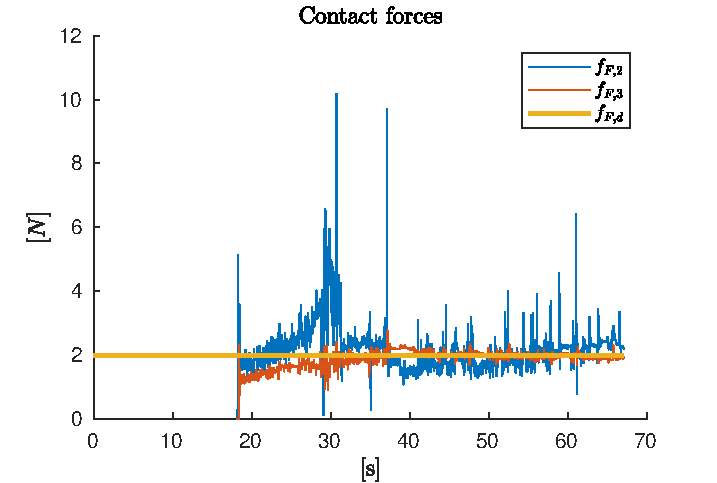
\includegraphics[width=0.9\textwidth]{figures/experiments/2xf/2xf-miniJ-forces.pdf}
    \caption{Contact forces from experiment with minimal CKCs}
    \label{fig:2xf-miniJ-force}
\end{figure}

Figure \ref{fig:2xf-miniJ-torque} shows the control torques of the snake robot. It is evident that in this case only the motors on joints 2, 3 and 4 are used. This is logical, as this is what the corresponding CKCs allow. Figure \ref{fig:2xf-miniJ-gazebo} show the configuration of the robot at the end of the simulation.

\begin{figure}
    \centering
    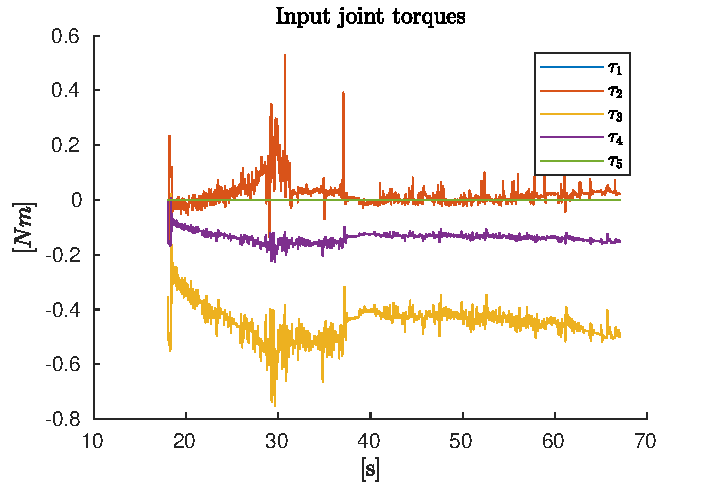
\includegraphics[width=0.9\textwidth]{figures/experiments/2xf/2xf-miniJ-torques.pdf}
    \caption{Control torques from experiment with minimal CKCs}
    \label{fig:2xf-miniJ-torque}
\end{figure}

\begin{figure}
    \centering
    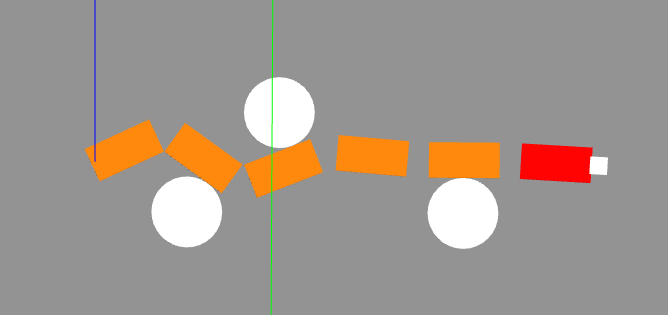
\includegraphics[width=0.8\textwidth]{figures/experiments/2xf/2force-gazebo.png}
    \caption{Snake robot configuration at the end of experiment with minimal CKCs}
    \label{fig:2xf-miniJ-gazebo}
\end{figure}

It should be mentioned that very thorough tuning of control parameters could improve the results, although a great deal of tuning already has been conducted. Furthermore, the control is quite twitchy as a result of the very varying force sensor feedback. Filtering the sensor signals with a low pass filter could have improved the smoothness of the results. However, the main sense of the experiment is still communicated with the presented results.

\subsection{Regular CKCs}

For the second simulation, the regular CKC formulations are used. By regular it is here meant that all contact points are described with respect to the base frame of the robot. This setup is illustrated in Figure \ref{fig:CKC1} in \ref{subsec:task-restrictions}. It can be seen that the two CKCs for the second and third obstacle are overlapping. As a result, the first two joint motors will be utilized to reach the control goal for both contact points. The motors for joints 3 and 4 will however still be reserved the third contact point. From Figure \ref{fig:2xf-bigJ-torque} it can be seen that all joint motors except for the last one are actuated. The last one is left out as it is in front of both the controlled contacts. 

Figure \ref{fig:2xf-bigJ-force} shows the resulting contact forces. As expected, the contact forces for the third contact point are much better controlled than for the second contact point. This is because it has more actuators available, again making it more robust. The actuators used for the second contact point are shared for both controls.

Another reason for why $f_{F,2}$ never reaches its desired value can be that the joint torques related to this control reach the saturation limit, which has an absolute value of 1. Unfortunately, it was found that larger motor torques easily led to the contact being lost at some moments. This is highly undesired as the mathematical model assumes contact at all times.

The end configuration of the snake robot after this simulation is shown in Figure \ref{fig:2xf-bigJ-gazebo}.

\begin{figure}
    \centering
    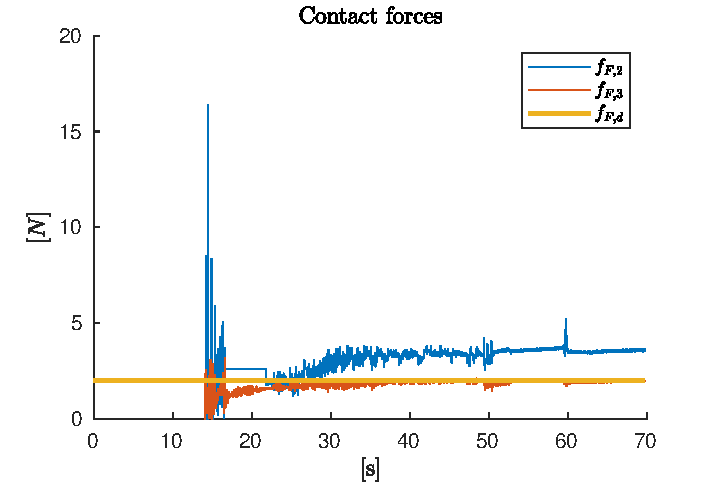
\includegraphics[width=0.9\textwidth]{figures/experiments/2xf/2xf-bigJ-forces.pdf}
    \caption{Contact forces from experiment with regular CKCs}
    \label{fig:2xf-bigJ-force}
\end{figure}

\begin{figure}
    \centering
    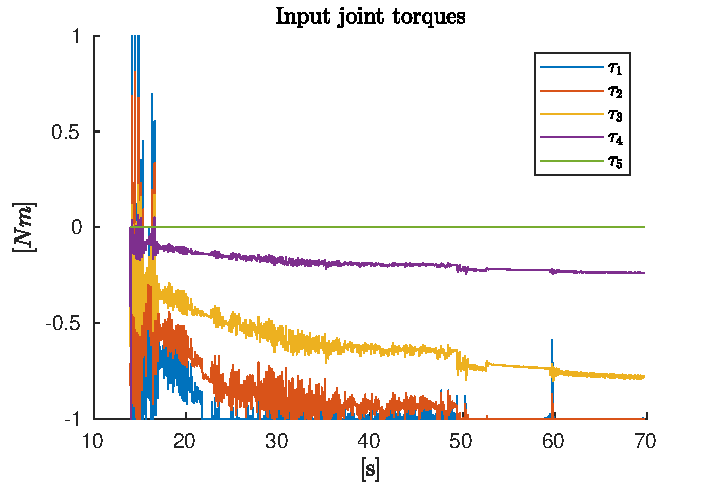
\includegraphics[width=0.9\textwidth]{figures/experiments/2xf/2xf-bigJ-torques.pdf}
    \caption{Control torques from experiment with regular CKCs}
    \label{fig:2xf-bigJ-torque}
\end{figure}

\begin{figure}
    \centering
    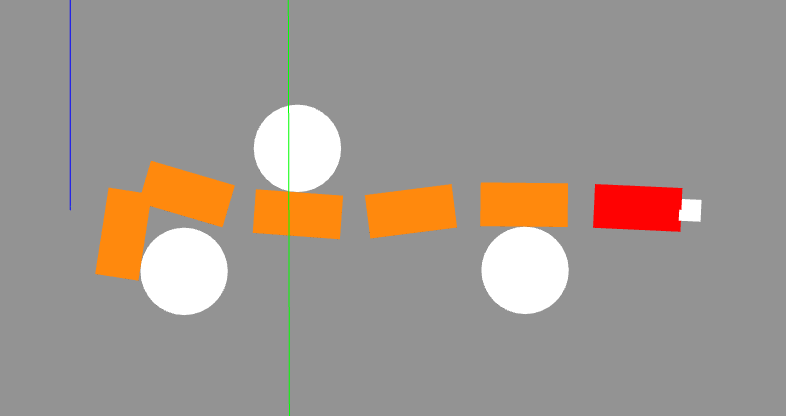
\includegraphics[width=0.8\textwidth]{figures/experiments/2xf/2force-bigJ.png}
    \caption{Snake robot configuration at the end of experiment with regular CKCs}
    \label{fig:2xf-bigJ-gazebo}
\end{figure}